\documentclass[fleqn]{article}
\usepackage{graphicx}
\usepackage{mydefs}
\usepackage{notes}
\usepackage{url}


\begin{document}
\lecture{Computer Vision}{HW05: Corner detection}{Name: Abhay Doke, UID: 29552668}

% IF YOU ARE USING THIS .TEX FILE AS A TEMPLATE, PLEASE REPLACE
% "CS 726, Fall 2011" WITH YOUR NAME AND UID.

Hand in via moodle at: \url{https://moodle.umass.edu/course/view.php?id=33024}.
Remember that only PDF submissions are accepted.  We encourage using
\LaTeX\ to produce your writeups.  See \verb+hw00.tex+ for an example
of how to do so.  You can make a \verb+.pdf+ out of the \verb+.tex+ by
running ``\verb+pdflatex hw00.tex+''.

% ANY LINE BEGINNING "%" IS A COMMENT.  YOU CAN UNCOMMENT THE BELOW
% TEXT AND FILL IN YOUR OWN.


\bee
\i The Harris corner detector computes the corner-score of a pixel as $f(\lambda_1, \lambda_2) = \lambda_1\lambda_2 - \alpha(\lambda_1 + \lambda_2)^2$, where $\lambda_1$ and $\lambda_2$ are the eigenvalues of the matrix M discussed in the class, and $\alpha$ is a parameter typically set $\in[0.04,0.06]$. In Matlab compute $f$ for $\alpha=0.04$ as a function of $\lambda_1$ and $\lambda_2$. The result should be a 2D image where the intensity of a pixel $(i,j)$ corresponds to $f(\lambda_1 = t_i, \lambda_2 = t_j)$. Uniformly sample a set of values of $t_i \in [0,1]$. You may find the $\texttt{meshgrid()}$ function in Matlab helpful for this. Use $\texttt{colormap jet}$ to display this image.



 \includegraphics[width=1\textwidth]{old.jpg}
 
\newpage

\i Come up with another function of $\lambda_1$ and $\lambda_2$ that might work as a corner score function. This function should be small when both values are close to zero, or when one value is significantly higher than the other. Plot this function next to the previous one.
\ene

My function of  $\lambda_1$ and $\lambda_2$ that might work as a corner function :
\[
\frac{2}{(\frac{1}{\lambda_1}) + (\frac{1}{\lambda_2})} + \alpha
\]

As seen in the plot below, this function is small when both values are close to zero, or when one value is significantly higher than the other. Plot is very similar to the original function.
 
 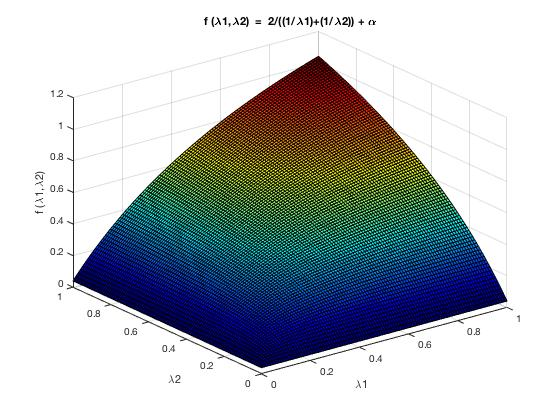
\includegraphics[width=0.9\textwidth]{new.jpg}


\end{document}
